\documentclass{article}
\usepackage[utf8]{inputenc}
\usepackage{graphicx}
\usepackage[russian]{babel}
\usepackage{amsmath}


\title{\textit{Лабораторная работа № 1}}
\author{Колесова Мария Николаевна}
\date{\today}

\begin{document}
\maketitle
\section{пример}
\subsection{формулы 1}
Создать формулу внутри строки $y = \sqrt[3]{x^3 + y^3}$. Следующая формула должна быть в отдельной строке $$y = \frac{x_1 + 1}{x_2 + 2}$$ но нельзя использовать окружение \textbf{equation}.

\vspace{\baselineskip}
\subsection*{Индексы}
\vspace{\baselineskip}

$x^{2y}$ $x^{2^{y}}$ $x_{y2}$ $x^{2n}_i$

$x^2_3 = x^2_3f``$
$$\int\limits_a^b ydy = h\sum_{i=1}^{n-1}y_i$$ и в строку $\int\limits_a^b ydy = h\sum_{i=1}^{n-1}y_i$

\vspace{\baselineskip}
\subsection*{Дроби}
\vspace{\baselineskip}

Деление на -n/2 дает (m + n)/n $$x = \frac{y^2 + z/3}{4 + \frac{y}{z + a}}$$

\vspace{\baselineskip}
\subsection*{Корни}
\vspace{\baselineskip}

$\sqrt[3]a\sqrt{a}$

\vspace{\baselineskip}
\subsection*{Размещение объектов друг над другом $\stackrel{=>}{A}$}
\vspace{\baselineskip}

\vspace{\baselineskip}
\subsection*{Матрицы}
\vspace{\baselineskip}
\begin{table}[h!]
    \centering
    $\left(
    \begin{tabular}{c c c}
       $a + x + y$ & $b$ & $4x$ \\ 
       x + y  & 2 + 5 & a + b \\ 
       x & $xz$ & -4 \\
    \end{tabular}
    \right)$
\end{table}

\vspace{\baselineskip}
\subsection*{Стиль}

$$x + \frac{1}{x + \frac{1}{x + \frac{1}{x + \frac{1}{x}}}}$$
\newpage
\subsection{формулы 2}
Далее следуют две формулы с использованием окружения \textbf{equation}.

Первая формула
\begin{equation}
    \begin{align*}
        &\dot{x} = ax - bx^2 - \frac{w_0xy}{x + d_0}, \\
        &\dot{y} = -cy + \frac{w_1xy}{x + d_1} - \frac{w_2yz}{y + d_2}, \\
        &\dot{z} = dz^2 - \frac{w_3z^2}{y+d_3},
    \end{align*}
\end{equation}

вторая формула
\begin{equation}
    \begin{aligned}
        \dot{x} = f(x) + \epsilon\sigma(x)\xi(t),
    \end{aligned}
\end{equation}

\newpage
\section{Таблица}
\begin{table}[h!]
    \centering
    \begin{tabular}{|c|c|c|c|c|}
        \hline
       \textit{a} is a bifurcation parameter  & b = 0.06 & w_0 = 1 & \multicolumn{2}{c|} {d_0 = 10} \\ \hline
       c = 1  & w_1 = 2 & d_1 = 10 & w_2 = 0.405 & d_2 = 10 \\ \hline
       d = 0.038 & w_3 = 1 & \multicolumn{3}{l|}{d_3 = 20} \\ \hline
    \end{tabular}
    \caption{Set of parameters}
\end{table}

\newpage
\section{Картинки}
Ниже идут 2 рисунка
\begin{figure}[h!]
    \centering
    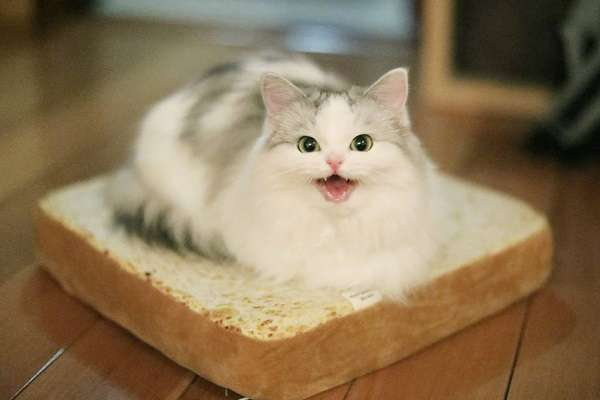
\includegraphics[scale=0.5]{cat.jpg}
    \caption{котенька}
    \label{fig:my_label}
\end{figure}
\begin{figure}[h!]
    \centering
    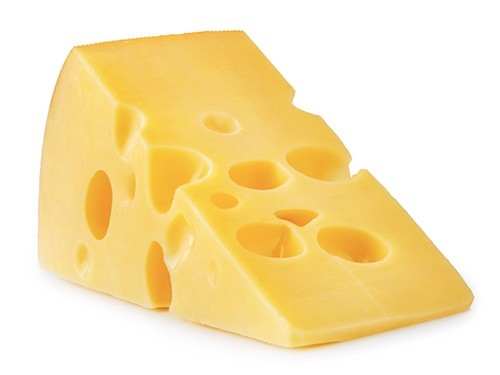
\includegraphics[scale=0.5]{cyr.jpg}
    \caption{это сыр}
    \label{fig:my_label}
\end{figure}

\newpage
\begin{equation}
    f(x) = \frac{A_O}{2} + \sum_{n=1}^{\infty}\lim_{x\to\infty} A_n \cos \left(\frac{2n \pi x}{\nu}-\alpha_n \right)
\end{equation}
( \big( \Big(\bigg( \Bigg( $$\xi$$

$\xi$
    $f(x)=a\cdot x + b$
\begin{figure}
    \centering
    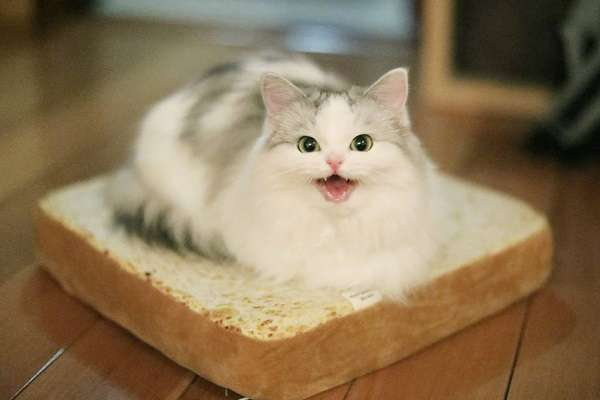
\includegraphics{cat.jpg}
    \caption{котенька}
    \label{fig:my_label}
\end{figure}

\begin{table}[h!]
    \centering
    \begin{tabular}{|c|c|}
        \hline
       A  & 1 \\ \hline
       B  & 2 \\ \hline
    \end{tabular}
    \caption{моя табличка}
    \label{tab:my_label}
\end{table}

\end{document}
